\subsection{Применение теории поля лигандов для описания химической связи в координационных соединениях переходных металлов}

Теория поля лигандов является производнои!от
теории кристаллического поля.
Метод молекулярных орбиталеи!и теория поля
лигандов
– это одно и то же.
Основные отличия теория кристаллического поля от
теории поля лигандов:
\begin{itemize}
\item Лиганд перестает рассматриваться бесструктурным,
становится структурирован со своими электронами.
Ранее электроны лиганда не рассматривались, только
заряд. Появляются представления о координационном
числе. Это число мест, занимаемых лигандом в
координационной сфере металла. Различают моно
- и
полидентантные лиганды.
\item Раз он структурирован, значит нужно смотреть, как
атомные орбитали металла перекрываются с
орбиталями лиганда. Если они перекрываются удачно,
то электроны взаимно делокализуются, а это ведет к
образованию энергетически выгодного состояния, то
есть, к связыванию.
\end{itemize}
Входя в комплексы, энергии орбиталей металла
повышаются. Рассмотрим на примере октаэдрических
комплексов:

\begin{itemize}
\item \textbf{Взаимодействие с лигандами сигма-типа}
\begin{figure}[H]
\centering
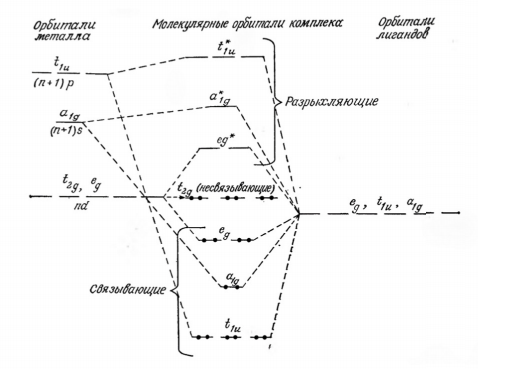
\includegraphics[scale=1.00]{images/TPL_sigma.png}
\end{figure}
Лопасти орбиталей $t_{2g}$ лежат между лигандами. Поэтому
перекрывание будет неэффективным, можно считать, что
они вошли в комплекс, не меняя энергии, относительно
сферически симметричного иона.
Орбитали $e_g$ и $t_{1u}$ направлены по осям к лигандам,
перекрывания будут хорошие.
В результате делокализации электронов стала больше
энергетическая щель между $t_{2g}$ и $e_g$. Перекрывание
орбиталей относится к ковалентным комплексам. В этом
случае комплексы должны быть низкоспиновые.
Поглощение сдвигается в сторону ультрафиолета, так что
окраска сдвигается в сторону бесцветных.
На уровне $s-$орбиталей можно провести уровень Ферми - такой уровень энергии, выше которого система не способна удерживать электроны. Если их будет более 18, система их отдаст. Это \textbf{правило 18 электронов}, и оно всегда будет пытаться реализоваться в ковалентных комплексах с хорошим перекрыванием.
О природе металла: если мы движемся по периоду слева
направо, количество электронов растёт, уровни орбиталей
ползут вниз.

\item \textbf{Взаимодействие с лигандами пи-типа}
Мы можем взять лиганд сложнее, там, где надо
учитывать пи
-взаимодействие. Пример перекрывания:
\begin{figure}[H]
\centering
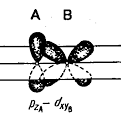
\includegraphics[scale=2.00]{images/pi.png}
\end{figure}
\end{itemize}

С помощью спектрохимического ряда можно определить, каким скорее будет пи-лиганд (пи-донорный или пи-акцепторный). Пи-акцепторные лиганды располагаются справа, пи-донорные слева.
\begin{itemize}
\item \textbf{Пи-акцепторные лиганды}
\begin{figure}[H]
\centering
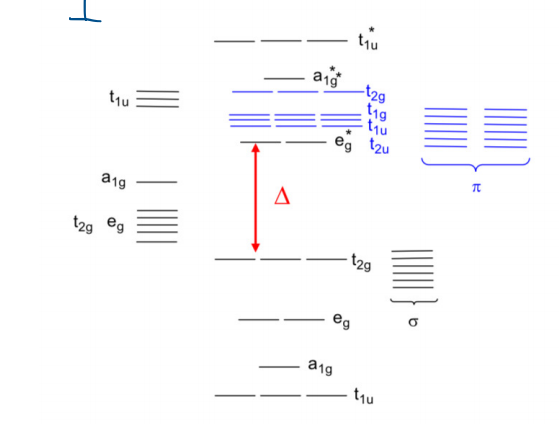
\includegraphics[scale=.750]{images/pi_accept.png}
\end{figure}
У таких лигандов пустые пи
-орбитали, они не могут
быть донором. Пустые орбитали всегда оказываются
выше по энергии. За счет взаимодействия с
p-вакантными орбиталями лиганда по энергии
понизятся орбитали $t_{2g}$ металла. Следовательно,
между $t_{2g}$ и $e_g^*$ увеличится энергетическое
расстояние, что увеличивает стабильность
комплексов. Поэтому таким комплексам выгоднее
быть низкоспиновыми. Соответствующие лиганды
относят к лигандам сильного поля.
\item \textbf{Пи-донорные лиганды}
\begin{figure}[H]
\centering
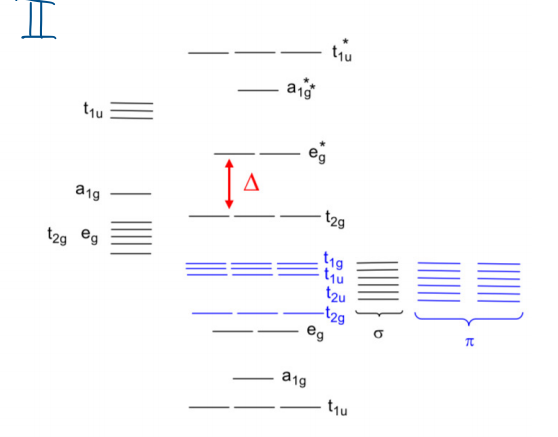
\includegraphics[scale=.750]{images/pi_don.png}
\end{figure}
Пи-орбитали заполнены электронами и находятся на
уровне сигма-орбиталей, но все - ниже d-орбиталей
металла. Наблюдается перекрывание $t_{2g}$ орбиталей, $t_{2g}$ орбитали металла поднимаются наверх, поэтому
уменьшается энергетическая щель между $t_{2g}$ и $e_g^*$. Характерны высокоспиновые комплексы.
Соответствующие лиганды относят к лигандам слабого
поля. 
\end{itemize}









